\subsection{Připojení databáze skrze ArcSDE}

Pro možnost připojení dat z databázového serveru PostgreSQL k produktům ArcGIS,
je potřeba nainstalovat PostgreSQL doplněný o knihovny ArcSDE. Instalační balík
lze stáhnout na {\it Esri Customer Care Portal
\footnote{https://customers.esri.com/}} a nainstalovat jej dle návodů dostupných na
{\it ArcGIS Resource Center
\footnote{http://resources.arcgis.com/en/help/main/10.1/index.html\#//002p000000t4000000}}.
U výběru verzí je nutné zajistit kompatibilitu verzí jednotlivých programů, viz kapitola \ref{kArcSDE}.

Po instalaci a konfiguraci PostgreSQL i knihoven ArcSDE je možno vytvořit
prostorovou databázi pomocí nástroje \texttt{Create Enterprise Geodatabase}
spuštěným na ArcGIS for Desktop (Standard nebo Advanced) nebo pomocí Python
skriptu. Takto lze existující databázi přidat schéma \texttt{sde}, které nese prostorové
funkce, indexy a datové typy, nebo vytvořit novou databázi s tímto schématem
\odkazObrazek{o}. ArcGIS produkty lze vždy připojit pouze k tabulkám, které jsou
uloženy ve schématu \texttt{sde}. 

  \begin{figure}[H]
    \centering
    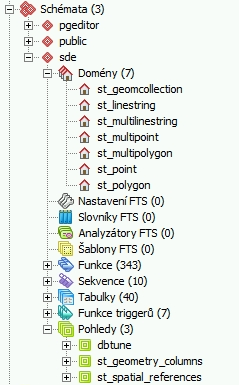
\includegraphics[scale=0.6]{../../../grafy/obr/sde_schema.png}
    \caption{Příklad struktury vytvořeného schématu sde}{Příklad struktury vytvořeného schématu \texttt{sde}}
          \label{o}
  \end{figure}

K databázi je poté možno se připojit obdobně jak u PostgreSQL. Přihlašovací
okno lze sputit pomocí ArcCatalogu, výběru Database Connections a volby
Database Connection, která otevře okno s možností zadání
přihlašovacích údajů \odkazObrazek{connect}. Pouze u první volby \texttt{Database Platform} je třeba vybrat jako databázového systém PostgreSQL. 

  \begin{figure}[H]
    \centering
    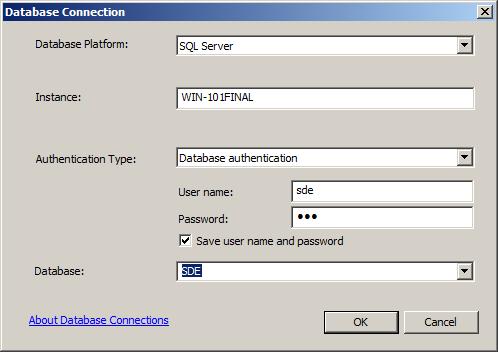
\includegraphics[scale=0.5]{../../../grafy/obr/conectScreen.png}
    \caption {Ukázka připojení databáze skrze ArcSDE}
          \label{connect}
  \end{figure}

